\documentclass[journal=jacsat,manuscript=article,layout=twocolumn]{achemso}
\usepackage[version=3]{mhchem} % Formula subscripts using \ce{}
\usepackage[T1]{fontenc}       % Use modern font encodings
% \usepackage[active]{preview}
%EXTRA PACKAGES%
% \usepackage{multicol}
\usepackage{xcolor}
\usepackage{textcomp}
\usepackage{geometry}
\usepackage[normalem]{ulem}

%%%%%%%%%%%%%%%%%%%%%%%%%%%%%%%%%%%%%%%%%%%%%%%%%%%%%%%%%%%%%%%%%%%%%
%% Place any additional macros here.  Please use \newcommand* where
%% possible, and avoid layout-changing macros (which are not used
%% when typesetting).
%%%%%%%%%%%%%%%%%%%%%%%%%%%%%%%%%%%%%%%%%%%%%%%%%%%%%%%%%%%%%%%%%%%%%
\newcommand*{\ga}{\alpha}
\newcommand*{\gb}{\beta}
\newcommand*{\gam}{\gamma}
\newcommand*{\gd}{\delta}
\newcommand*{\eps}{\epsilon}
\newcommand*{\veps}{\varepsilon}
\newcommand*{\gz}{\zeta}
\newcommand*{\gt}{\theta}
\newcommand*{\gi}{\iota}
\newcommand*{\gk}{\kappa}
\newcommand*{\gl}{\lambda}
\newcommand*{\gs}{\sigma}
\newcommand*{\go}{\omega}
\newcommand*{\Gam}{\Gamma}
\newcommand*{\gD}{\Delta}
\newcommand*{\gT}{\Theta}
\newcommand*{\gL}{\Lambda}
\newcommand*{\gS}{\Sigma}
\newcommand*{\gO}{\Omega}
\newcommand*{\pt}[1]{\left( #1\right)}
\newcommand*{\pq}[1]{\left[ #1 \right]}
\newcommand*{\pg}[1]{\left\{ #1\right\}}
\newcommand*{\figref}[1]{\figurename~\ref{#1}}
\newcommand*{\red}[1]{\textcolor{red}{#1}}
\newcommand*{\blue}[1]{\textcolor{blue}{#1}}
\newcommand*{\gray}[1]{\textcolor{gray}{#1}}
% \renewcommand{\baselinestretch}

%%%%%%%%%%%%%%%%%%%%%%%%%%%%%%%%%%%%%%%%%%%%%%%%%%%%%%%%%%%%%%%%%%%%%
%% Meta-data block
%% ---------------
%% Each author should be given as a separate \author command.
%%
%% Corresponding authors should have an e-mail given after the author
%% name as an \email command. Phone and fax numbers can be given
%% using \phone and \fax, respectively; this information is optional.
%%
%% The affiliation of authors is given after the authors; each
%% \affiliation command applies to all preceding authors not already
%% assigned an affiliation.
%%
%% The affiliation takes an option argument for the short name.  This
%% will typically be something like "University of Somewhere".
%%
%% The \altaffiliation macro should be used for new address, etc.
%% On the other hand, \alsoaffiliation is used on a per author basis
%% when authors are associated with multiple institutions.
%%%%%%%%%%%%%%%%%%%%%%%%%%%%%%%%%%%%%%%%%%%%%%%%%%%%%%%%%%%%%%%%%%%%%
\author{Elizaveta Guseva}
\email{elizaveta.guseva@stonybrook.edu}
\affiliation[Stony Brook University]
{Laufer Center for Physical and Quantitative Biology, Stony Brook University, Stony Brook, NY, (United States)}
% \altaffiliation{A shared footnote}
\author{Ronald N Zuckermann}
\affiliation{Lawrence Berkeley National Laboratory (LBNL), Berkeley, CA (United States)}
\author{Ken A Dill}
\email{dill@laufercenter.org}
\phone{+1631 632 5400}
\fax{+1631 632 5405}
\affiliation[Stony Brook University]
{Laufer Center for Physical and Quantitative Biology, Stony Brook University, Stony Brook, NY, (United States)}


%%%%%%%%%%%%%%%%%%%%%%%%%%%%%%%%%%%%%%%%%%%%%%%%%%%%%%%%%%%%%%%%%%%%%
%% The document title should be given as usual. Some journals require
%% a running title from the author: this should be supplied as an
%% optional argument to \title.
%%%%%%%%%%%%%%%%%%%%%%%%%%%%%%%%%%%%%%%%%%%%%%%%%%%%%%%%%%%%%%%%%%%%%
\title[]
  {How random prebiotic polymers could grow long and informational}

%%%%%%%%%%%%%%%%%%%%%%%%%%%%%%%%%%%%%%%%%%%%%%%%%%%%%%%%%%%%%%%%%%%%%
%% Some journals require a list of abbreviations or keywords to be
%% supplied. These should be set up here, and will be printed after
%% the title and author information, if needed.
%%%%%%%%%%%%%%%%%%%%%%%%%%%%%%%%%%%%%%%%%%%%%%%%%%%%%%%%%%%%%%%%%%%%%
\abbreviations{IR,NMR,UV}
\keywords{American Chemical Society, \LaTeX}

%%%%%%%%%%%%%%%%%%%%%%%%%%%%%%%%%%%%%%%%%%%%%%%%%%%%%%%%%%%%%%%%%%%%%
%% The manuscript does not need to include \maketitle, which is
%% executed automatically.
%%%%%%%%%%%%%%%%%%%%%%%%%%%%%%%%%%%%%%%%%%%%%%%%%%%%%%%%%%%%%%%%%%%%%



\begin{document}
\abstract{\footnotesize How living systems arose prebiotically from random physical-chemical 
processes is a
longstanding question. When did undirected(??) chemical reactions begin to capitalize on
fitness and undergo Darwinian evolution? 
Many origins-of-life studies are post-informational (postbiotic), i.e. focusing on
processes that happen after there is already a molecular code and an ability to
propagate ``self''.
Here, in contrast, we are focusing on the transition from prebiotic to postbiotic.
We are interested in how polymers with random sequences may lead to informational
polymers with particular sequences, which then dominate the population. To study
sequence-structure properties of informational copolymers we use HP lattice model --
a successful polymer-folding model of hydrophobic (H) and polar (P) monomers. 
Using sequences and structural information from the HP-model we have found
conditions under which a set of certain sequences dominates the population with time.
We use direct stochastic simulations of the dynamic models of the polymerization to
figure out how sequence structure and aspects of the different dynamic models
determine the structure and behavior of the emerged cooperative sets of the
polymers. We find that some sequences become autocatalytic for accelerating the
syntheses of others.}

%%%MAIN TEXT%%%%

 
\section{Introduction} 

We are interested in two important puzzles about the early origins of life: How might prebiotic polymerization 
processes have produced long chains of protein-like or nucleic-acid-like molecules?  And, how 
could random processes acting on random sequences have led to early sequence-structure relationships~\cite{Joyce1987,Abel2005}?

We know that amino acids can be produced prebiotically \cite{Miller1953} and are abundant in 
stony meteorites \cite{Sephton2002} and significant progress has been made in synthesis of 
single nucleotides \cite{Powner2009a}.
Furthermore, many experiments show that both amino acids and nucleotides can be polymerized into 
short chains under prebiotic conditions without 
the presence of enzymes
\cite{Shock1992,Martin1998,PAECHT-HOROWITZ1970,Lambert2008,Leman2004a,Orgel2004,Ferris1996}.  
It is as well known that the yields of such short-chain oligomers can be increased under 
prebiotically plausible conditions by such processes as adsorption to 
clays\cite{Rao1980,Lambert2008} or minerals\cite{Bernal1949,Ferris1996}, by evaporation of tidal 
pools\cite{Nelson2001}, by concentration in ice through eutectic melts \cite{Kanavarioti2001} or 
freezing\cite{Bada2004} or temperature cycles. 

It remains a conundrum, however, how prebiotic processes could have overcome what we call the 
``Flory Problem''. It is generally assumed that the minimum chain lengths of proteins or nucleic 
acids required for formation of complex structures essential for function estimated to be around 
30-60 monomers long \cite{Szostak1993}. 
Yet, known mechanisms  of polymerization lead to polymers, which 
concentrations drop exponentially as their chain length increases.   
 Therefore it appears impossible to generate viable amount of long enough chains in prebiotic 
synthesis. As an illustration, we list here several experimental studies on prebiotic 
polymerization of amino acids and nucleotides. Leman et al. showed that carbonyl sulfide (COS), a 
simple volcanic gas, brings about the formation of oligo-peptides from amino acids under mild 
conditions in aqueous solution in minutes to hours. But the product is mainly dimers and 
trimers~\cite{Leman2004a}.  In another study, using various mineral catalysts such as calcium 
montmorillonite, hectorite, silica or alumina, mixtures of Gly and Gly$_2$ grow to about 6-mers 
after 14 days~\cite{Rode1997,Rode1999}.  Or, by freezing samples of phosphoimidazolide-activated 
uridine in the presence of metal ions in dilute solutions, Kanavarioti found polymers of 
oligouridylates up to 11 bases long, with an average length of 4 \cite{Kanavarioti2001}.  And, 
starting from decanucleotides [$^{32}$P]dA(pdA)$_8$pA adsorbed on Na$^+$-montmorillonite, Ferris et 
al. observed chains averaging lengths 20-40 after 14 days at 25\textcelsius\ \cite{Ferris1996}.  It 
is not yet understood how prebiotic polymerizations could lead to the types of long protein or 
nucleic-acid chains in present-day cells.

   
\section{The Flory problem of obtaining long chains}
\label{sec:flory} 
The standard processes of chain polymerization lead to the the Flory or Flory-Schulz distribution of the concentrations of chains of different chain lengths~\cite{Flory1953}. 
\begin{equation}
 f(a)=a^2l(1-a)^{l-1},
\end{equation} 
where $l$ is the chain length and $a$ is the probability of chain termination, which is a measure of the average chain length: $\langle l \rangle = a(2- a)$.
Figure \ref{fig:flory} shows the central prediction of Flory theory, that longer chains are exponentially less populated than shorter chains.  For example (see the blue line in Fig~\ref{fig:flory}):
\begin{equation}
  \frac{\pq{10~\mathrm{mers}}}{\pq{1~\mathrm{mers}}}\propto10^{-4},\qquad\frac{\pq{20~\mathrm{mers}}}{\pq{1~\mathrm{mers}}}\propto10^{-9}
\end{equation} 
Thus, for a synthetic process that starts with micro-molar concentrations of monomers, the 
average chain length would be $\langle l \rangle = 2$ and 40-mers would have 
negligible concentrations of $\propto 10^{-19} $ mol/L. 
\begin{figure}[h!]
  \centering
  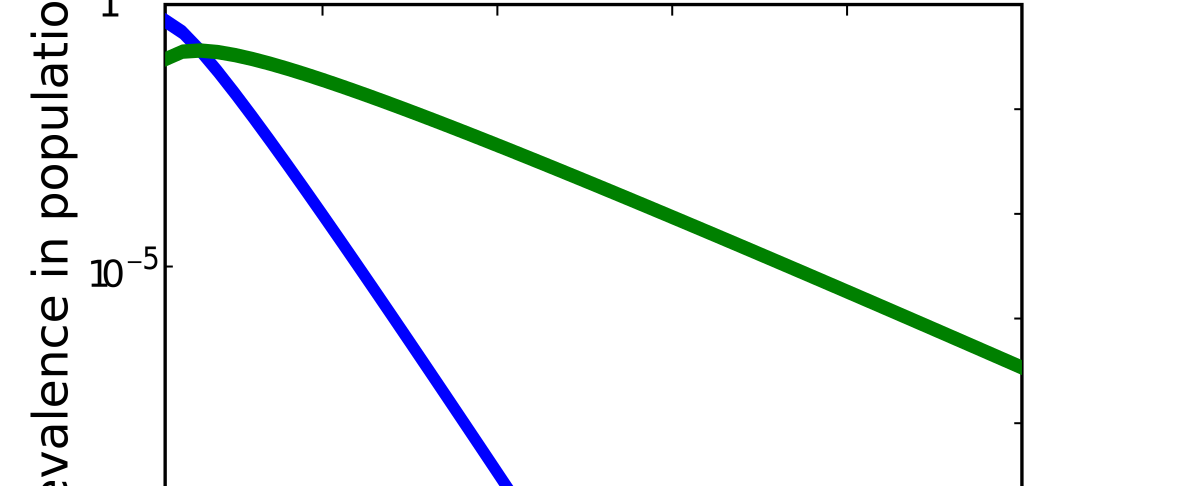
\includegraphics[width=\columnwidth]{pictures/flory2.pdf} 
  \caption{The Flory length distribution that arises from spontaneous polymerization processes.}
  \label{fig:flory}
\end{figure}

\red{E -- I don't understand what these following refs are saying, and how it relates to our 
point.}

 \blue{Ken - The ref in the paragraph below, talks about insufficiency of increasing of 
polymerization constant. They say the dynamics of the system must be changed in order to get rid of 
exponential distribution. And we introduce a physical principle, which we claim changes the 
dynamics}

 While increasing equilibrium constant by means of catalysis or 
changing conditions to dry medium would lead to longer chain lengths, it will still give 
exponentially decreasing distribution of length\cite{Derr2012}. 

The Flory distribution is a good model of prebiotic syntheses of peptide and nucleic acid chains 
(see Figure~\ref{fig:some_flory}), although in some cases a very similar exponential law, 
$f(a)\propto const^l$ applies instead\cite{nowak2008prevolutionary,Derr2012}.  A consequence is 
that since prebiotic chemistry appears to give submillimolar or submicromolar concentrations of 
monomers, it has been expected that longer chains would be present in negligible 
concentrations~\cite{Aubrey2009,Kanavarioti2001,Lazcano1996}.

\red{E - You mean $(1-a)^l$, rather than $a^l$?}

\blue{Ken - I changed to ``const'' so that ``a'' doesn't acquire extra meaning.}

\begin{figure}[h!]
  \centering
  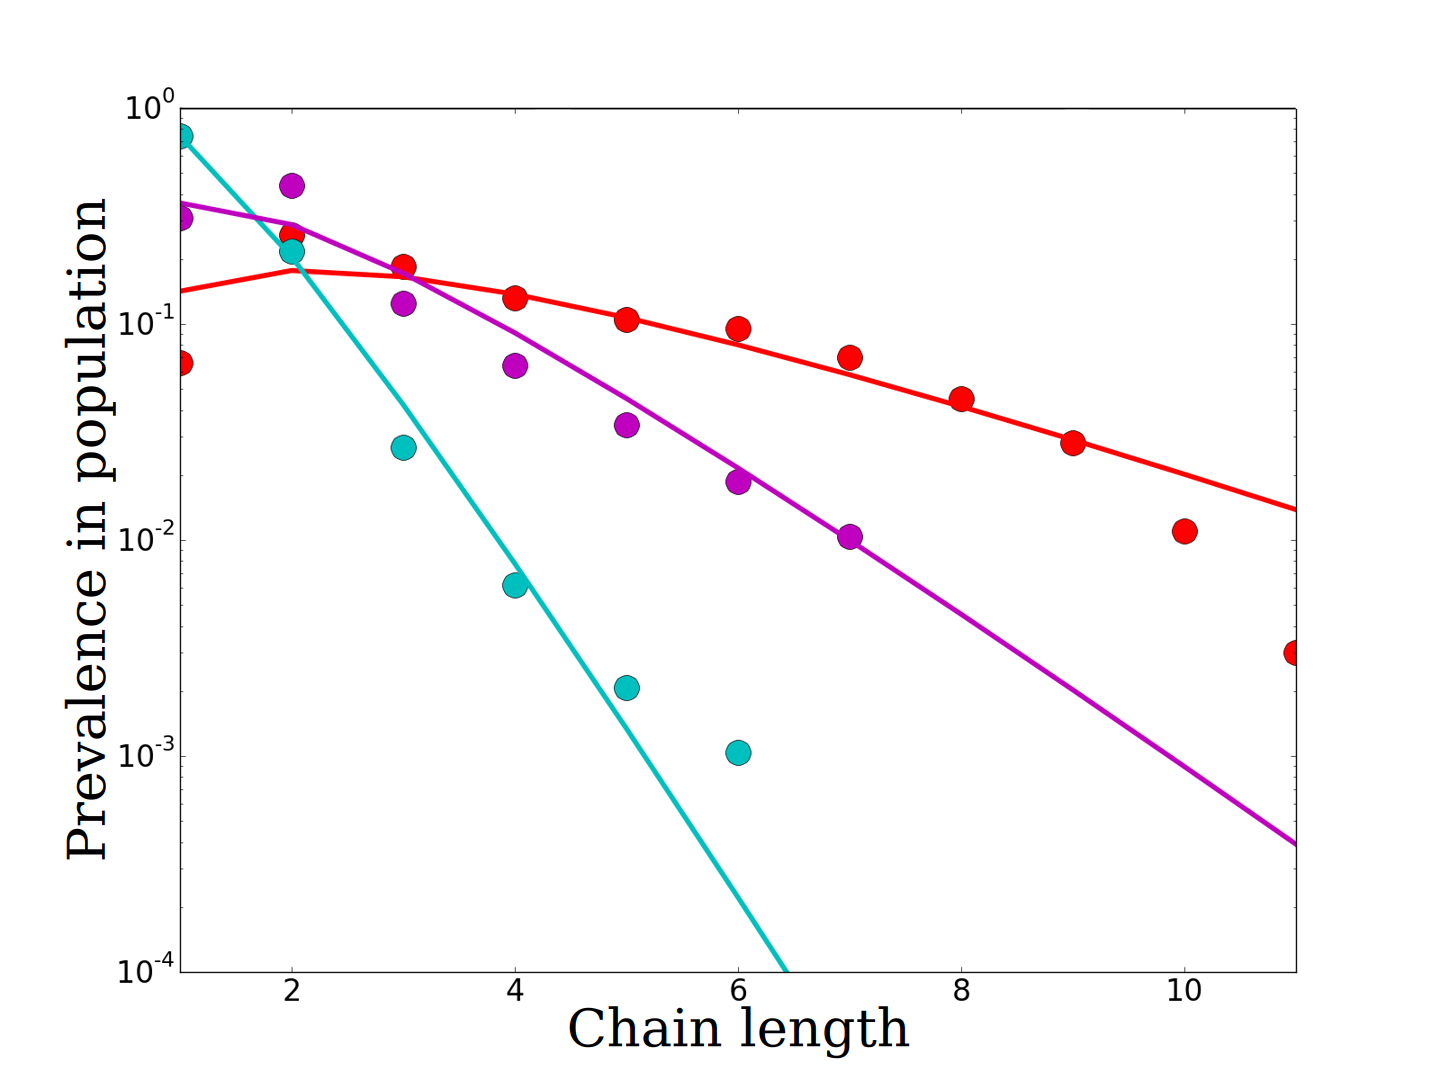
\includegraphics[width=\columnwidth]{pictures/some_flory.pdf} 
  \caption{Chain-length distributions of peptides and nucleic acids synthesized under prebiotic 
conditions.  The lines show curve fits to the Flory distribution for polymerization processes. Data 
points: red -- Kanavarioti\cite{Kanavarioti2001}, cyan -- Ding\cite{Ding1996}, 
magent -- Ferris\cite{Ferris1999}}
  \label{fig:some_flory}
\end{figure}




\section{The foldabilities of random HP polymers can give a sequence-structure code}
\blue{Ken -- are you sure that this is a good section name? }

We show here that random short sequences of hydrophobic and polar monomers (called HP polymers): (i) 
can fold to compact structures, leading to sequence-structure relationships even in solutions of 
random sequences.  And, (ii) that some folded HP sequences may be catalytic and autocatalytic, 
leading to a selection mechanism for escaping the Flory Problem.  

The conformations and sequences of HP polymers have been studied extensively as a model for the 
folding and evolution of 
proteins\cite{lau1989lattice,Chan1991,Miller1995,Yue1995,agarwala1997local}.  Such studies have 
shown that the sequence-structure relationship of proteins is to a large extent a result of 
hydrophobic-polar sequence patterning [  ].  They have further demonstrated that a large fraction 
of the space of random sequences can collapse into compact structures resembling native proteins [  
]; see fig. 
\ref{fig:hydro-effect}.  This code is not critically dependent on the chemical details of the 
monomers, so about half of the 20 amino acids classify as H and about half as P.  And, we note below 
in more detail that RNA molecules can also fold in water, indicating differential solvation, so our 
analysis below is not limited to proteins as foldamers.

\begin{figure}[h!]
  \centering
  \includegraphics[width=\columnwidth]{pictures/hp-model.pdf} 
  \caption{HH interactions are favorable in water, leading to different compact states for different 
HP sequences.}
  \label{fig:hydro-effect}
\end{figure}

\marginpar{E - I favor a slightly different figure here.  First, let's show 2 different sequences, 
each leading to its unique native state.  Second, let's a more interesting HP sequence for each of 
the two sequences.  For the present one, most of the polar monomers will be flopping around, not 
defining a native state.}

\section{HP polymerization studied using a HP modified Nowak (HPN) model}

We consider a dynamical process in which at any given time step: a monomer can add to a growing 
chain with rate xx; the polymer can be degraded with rate yy; ... [give essentials here concisely, 
keep the details in the SI.]  This model was developed by Nowak and colleagues and applied to 
homopolymerization.  Here, we modify it for our HP heteropolymers, as follows ....  [We added 
non-zero hydrophobic energy and introduced folding and unfolding reactions.  The hydrophobic energy 
is taken to be $E_h=2kT$ and the rate of unfolding is $k_{unf}=100$.]


\section{HP folding alone does not solve the Flory Problem}

Figure~\ref{fig:sim.flory-fold} shows the result of our application of the HPN model to random HP 
polymers.  In short, it shows that folding alone does not substantially modify the Flory chain 
length distribution.  Here's why ... Here's how folding is assumed to affect the chain-length 
distribution in the HPN model...   This conclusion is independent of the parameters chosen, over a 
wide range (results not shown).

\begin{figure}[h!]
  \centering
  \includegraphics[width=\columnwidth]{pictures/flory-and-fold.pdf} 
  \caption{Dashed lines represent polymerization without folding or catalysis. Solid lines 
correspond to simulations run with folding but without catalysis. For details of simulations see 
section \ref{sec:mat-sim}, Experiment 2. }
  \label{fig:sim.flory-fold}
\end{figure}

\section{Some HP-foldamers can also be catalysts}

Since present-day proteins can catalyze reactions -- including the reaction that synthesizes the 
peptide bond -- it is not hard to imagine that some primitive foldamers could have had some 
primitive catalytic capability.  A typical enzyme catalyzes its reaction using just a few critically 
positioned amino acids.  For example, serine proteases utilize a catalytic triad of 3 amino acids [ 
; other examples ...].  Here, we use a toy model to capture that simple idea, namely that a folded 
polymer can position a small number of residues in a way that can catalyze a reaction.  

Fig. \ref{fig:hp-catalysis} shows the idea.  Suppose a polymer molecule $A$ folds in such a way as 
to provide a surface with a few hydrophobic amino acids.  Suppose that surface serves as a sticky 
spot for another HP molecule $B$ adjacent site a sticky spot for an H monomer $C$ that could add to 
polymer $B$.  This binding to the catalyst $A$ of both chain $B$ and monomer $C$ would then give a 
positional localization that reduces the kinetic barrier for polymerization.  A typical hydrophobic 
interaction is $1-2kT$.  So chain $A$ is a catalyst that could simply provide a hydrophobic landing 
pad, reducing the rate barrier by 3-4 hydrophobic interactions, thereby increasing the 
polymerization rate by $\approx 100$-fold (fig.\ref{fig:hp-catalysis}(b)).  Of course, this rate 
enhancement is much smaller than the $2\cdot10^7$-fold of modern ribosomes~\cite{Sievers2004a}. But, 
it gives a conceptual basis for how peptide-bond formation rate enhancements could have begun 
prebiotically.

Before proceding further, we note what is intended and what is not intended from this model.  This 
model is not intended as an accurate model of any real catalytic mechanism.  Rather, it is a toy 
example of only one possible mechanism.  In this case, the mechanism is simply translational 
localization of the two reactants, polymer $B$ and monomer $C$ for extending the chain.  At the 
present time, this coarse-grained simplification is the only unbiased and practical type of model 
that can estimate the size of protein sequence space relevant for such catalysis.

\begin{figure}[h!]
  \centering
  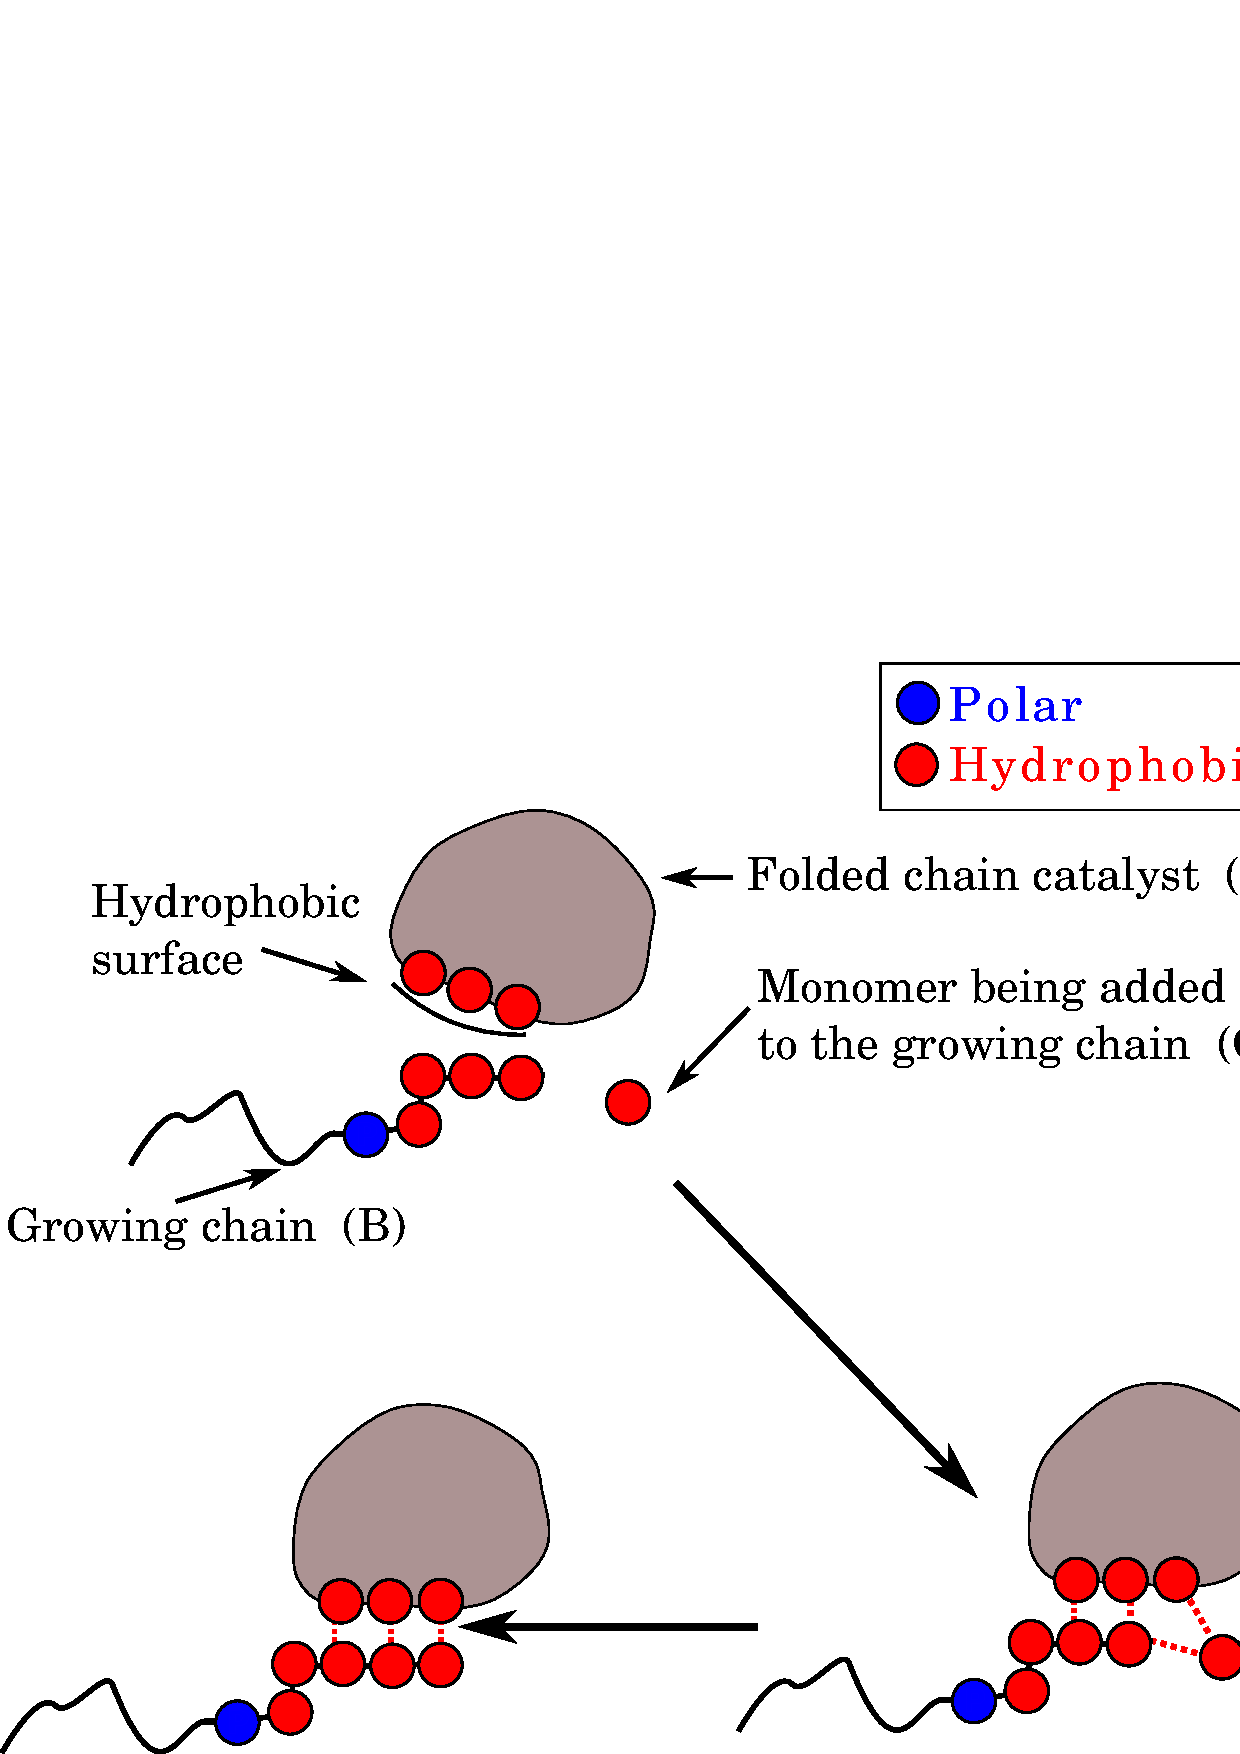
\includegraphics[width=0.9\columnwidth]{pictures/hp-catalysis.pdf} 
  \caption{Catalyst catalyzes a growing of an unfolded hp-polymer. 
           Having just 3-4 hydrophobic contacts is enough to lower an 
           activation barrier for $\propto 100$ times at room 
           temperature.}
  \label{fig:hp-catalysis}
\end{figure}


\subsection{HP foldamer-catalysts can solve the Flory Problem}

Figure~\ref{fig:sim.flory-fold} shows the HPN model, now allowing for both the folding of all HP 
sequences, according to the rules of the HP model, and allowing for catalysis based on all those 
foldamers that have xxx H monomers on their surfaces in their unique native folded states (see SI 
for details).  This figure makes a key point of this paper, namely that the catalysis that results 
from some foldamers -- even though it is weak -- can lead to solving the Flory Problem.  Accounting 
for the folding and catalysis of some HP sequences (unbroken red line) shows that the populations of 
25-mer chains, in the model estimation, will be about 6 orders of magnitude higher than when not 
accounting for folding and catalysis.  And, that amplification factor increases for longer chains.  
More tests and details are given in the SI.

\begin{figure*}[h!]
  \centering
  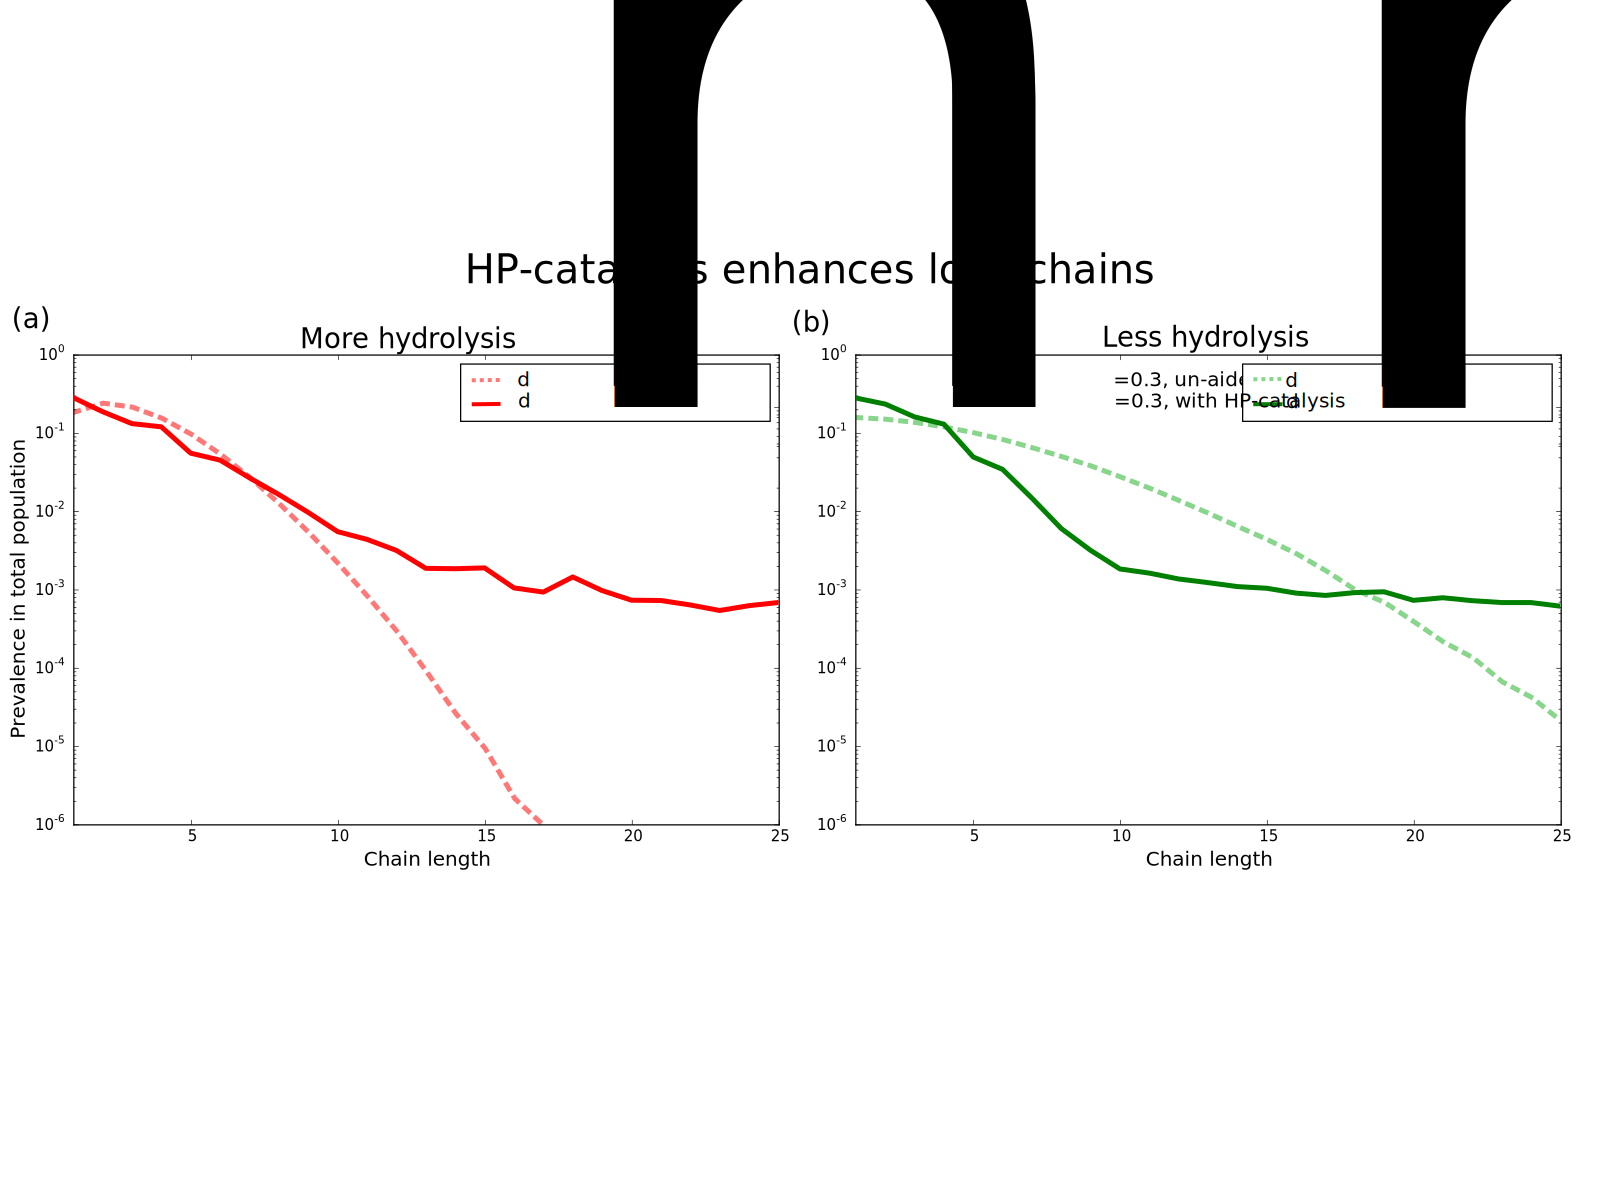
\includegraphics[width=0.95\textwidth]{pictures/flory-and-hp.pdf} 
  \caption{Dashed lines represent polymerization without folding or catalysis. Solid lines 
correspond to simulations run with folding and catalysis. For details of simulations see 
section \ref{sec:mat-sim}, Experiment 2. }
  \label{fig:sim.flory-fold}
\end{figure*}

\marginpar{E - Let's just keep fig a here, and move fig b to SI.  -- Also, can we expand the y-axis, 
so that we can show what happens to the red dashed curve for chain length 25?  I've tried to 
estimate this in the text above.}

\section{HP foldamer catalysts give a structural basis for autocatalysis}

 It has long been recognized that the origin of life requires some form of 
autocatalysis~\cite{Kauffman1986,Dyson1985,Eigen1978}.  But, as far as we know, no molecular 
structural mechanism has yet been proposed [E - is that true?].  The present work gives such a 
structural mechanism: a random short HP polymer $A$ folds and catalyzes the elongation of another HP 
polymer $B$, which, in turn elongates $A$.  We found these sequences as we sought an explanation for 
the results of Figure~\ref{fig:sim.flory-fold}.  Some of the sequences and folds of these autocats 
are shown in Figure~\ref{fig:example1}.


\begin{figure}[h!]
  \centering
  \includegraphics[width=\columnwidth]{pictures/good_seqs.pdf} 
  \caption{Some examples of dominating autocatalytic sequences. Gray lines represent regular 
non-catalytic sequence. structures on the right are native structures of autocatalytic sequences. }
  \label{fig:example1}
\end{figure}
% \newline

\marginpar{E - We need a better fig here.  Here are 3 folded structures.  But, we are not showing 
their autocat partner.  Can we show those?  And, can we indicate how the A folds the B and how the B 
folds the A?}


 The autocat sequences we find are only a small fraction of sequence space.  On the one hand, 
sequences that have too many P residues don't fold well, and also will be hydrolyzed rapidly.  On 
the other hand, sequences that have too many H residues don't fold to unique native states; they 
have many compact oil-droplet structures.  And, they will aggregate.  Our model supposes that only 
relatively unique folds are stable over long enough times to be able to bind and catalyze reactions. 
 So, we tend to find the autocats have HP compositions within the range of $50-80\%$ hydrophobic 
monomers.
 

\section{Discussion}


Here are some examples of other models using autocatalytic sets
\begin{itemize}
 \item Several studies\cite{Eigen1978,Dyson1985,Kauffman1986} focused on how such self-sustaining 
systems could work if they already exist. They investigated under which conditions these systems 
indeed are self-maintaining.

\item In a more recent series of works \cite{segre1998graded,Segre2000,Markovitch2012} 
 authors numerically studied auto and cross catalysis in an artificial chemical system of 
 small mutually catalyzing  molecules. They found parameters of the system for which one can 
observe 
diversity and replication fidelity.
 Appearance of these desirable properties requires high mutual catalysis propensity.

\item In \cite{Tkachenko2014} authors studied random heteropolymers capable of template 
assisted ligation and random breakage. In such a system, they showed,  long-chained
polymers  can be sustained by the mutual catalysis of the ligation reaction. They discovered
that a system with ligation and hydrolysis is capable of first order phase transition, depending 
concentration. 
In their system the maximum length of heteropolymers is determined kinetically as a simple function 
of the ratio
between ligation and breakage rates

\item In \cite{Walker2012} authors considered a system with finite monomer source, spontaneous 
reversible polymerization
and template ligation of binary polymers. With stochastic simulations, they studied how kinetic 
rates of polymerization/degradation
affect ability of sequences to explore sequence space. Similarly to our results, the higher the 
ratio of degradation rate
over polymerization rate (in our case (hydrolysis and hydrophobic energy), the higher the diversity 
of the pool, and the lower it, the higher number of functional sequences is observed (functional 
polymers are randomly assigned). Functional sequences are able to emerge spontaneously,
they don't dominate the pool, allowing for further pool exploration. While \cite{Walker2012} and our 
system are kinetically different they experience rather similar dynamics.
\end{itemize}

Many studies focused on how in a particular situation autocatalytic systems could arise and on 
different properties of the emergent results based on type of autocatalytic mechanisms.
\begin{itemize}
\item The idea of 
autocatalysis was applied by Wu and Higgs\cite{Wu2009} to homo-polymers: while system of 
homopolymers cannot be 
complex and capable of storing information, authors showed that their system has bi-stability and 
increased proportion of long polymers.
 \item In a series of works \cite{nowak2008prevolutionary,Ohtsuki2009,Chen2012,Derr2012} 
 authors investigated binary polymers 
either capable of autocatalysis or replication. They showed that while autocatalytic system has 
bi-stability and increased ratio of longer polymers, one has to increase catalysis rate 
exponentially in order to get exponential growth of longer chains. Self-replication system on the 
other hand didn't show bi-stability, but on a positive side, relatively low replication rate 
constant brought up significant growth of longer polymers. It was also shown that self-replication 
enhances complexity of the system. The autocatalysis mechanism of this series is however very 
simple It's a self-replication performed by means of catalysis: for every reaction catalyst has to 
get attached to a growing molecule and then dissociate from it.


Significant progress has been made in attempts to make artificial autocatalytic sets in a 
laboratory\cite{VonKiedrowski1986,Lincoln2009,Vaidya2012}. These experiments, while working with 
simple artificially designed systems, exhibit a nice example of original principle.


They key difference with our work is 
that hydrophobic interaction provides a simple physical set up which produces non-linear dynamics 
with complex feedback.
This enables system to develop a non-trivial selection mechanism. Our system, as being based on 
\cite{Ohtsuki2009} model, experience bi-stability, has semi-periodic fluctuations  
and polynomial length distribution \red{??} 
\end{itemize}

\red{
\begin{itemize}
 \item Hordijk2010.
\end{itemize}
}


\subsection{2D-3D}
\begin{itemize}
 \item Folding and unfolding rates are likely underestimated in 2D case
 \item Overall length dependence is steeper in 2D case
 \item However cases are very similar and it's possible to do a mapping between them: there's a 
direct mapping between surface to volume ratio in 3D case to perimeter to area ratio in 2D case
\end{itemize}


\section{Materials and methods}\label{sec:mat}
\subsection{Simulations}\label{sec:mat-sim}
To test our hypothesis we performed direct stochastic simulations on several sets of parameters. We 
used 
\blue{PDMmod} method \cite{Bernatskiy}
% \footnote{C++ library and description can be found here: https://github.com/abernatskiy/pdmmod}. 
Stochastic simulations keep track of each 
molecular specie in the system. However simulations are limited due to computational reasons. 
First 
of all we have to explore conformational space of every polymer. This task is NP-hard (we use 
HPSandbox algorithm\cite{lau1989lattice,Dill2008} \footnote{Python implementation and description 
can be found here: http://hp-lattice.readthedocs.org/en/latest/}), so we had to limit 
maximum chain lengths to 25. We also try to keep total number of species in the low thousands, to 
avoid computational costs. We do it by introducing dilution parameter $d$: molecules are being 
removed from the system with probabilities $\propto d$. 
This either can mimic a protocell splitting and loose of materials due to it or in the case when 
system isn't bounded by any borders the fact that some molecules will diffuse away. Total number of 
molecules varies from simulation to simulation, 
however it mostly holds in the region \red{insert}.

We start our simulations with a small pool of monomers, usually below 100 molecules. 
\begin{itemize}
 \item We assume that there are enough of activated monomers in the system, so that their 
concentrations are constant. This way we don't have to track them in the simulations.

\item Polymers can therefore spontaneously grow with the rate $\ga$. Without loss of generality we 
can put this parameter equal 1; all other rates with be relative to the growth rate in this case.

\item Hydrolysis has constant rate $d_h$ per bond. Half-life time of hydrolysis bonds in neutral 
conditions and temperatures around room temperature are on the order of hundreds of 
years\footnote{Hydrolysis rate constants of oligopeptides in 
neutral conditions are of the order of $10^{-11}-10^{-10}$: $1.3  10^{-10} M^{-1}s^{-1} $ 
for benzoylglycylphenylalanine ($t_{1/2} = 128 y$)\cite{Bryant1996}, $6.3  10^{-11} M^{-1} s^{-1}$
($t_{1/2}=350 y$) for glycylglycine and $9.3 10^{-11}M^{-1} s^{-1}$ for glycylvaline
\cite{Smith1998}.}. We test hydrolysis rate constants to be about $0.001-1$ of polymerization rate 
constants. This way we account for polymerization conditions, which happens on the order of days 
to years.

\item We also import monomers into system with rate $a\gg1$. It is safe to assume that we would 
have enough monomers in the system and import of monomers wouldn't be a bottleneck of reactions 
chain. Therefore we explore big values of $a\propto 
10^2,10^3\ga$

\item Dilution parameter $d$ mimics cell division and loss of the matter because of that. From 
\ref{sec:nowak-steady} we see that total mass of the system is  $ M\propto\frac{a}{\ga}, \qquad 
d\approx \ga\quad \mbox{or}\quad d\gg \ga$ and $M\propto \frac{a}{\ga}\frac{d}{2\ga} ,\qquad 
d\ll\ga$. Therefore we explore valued of $d$ from $\propto 0.01\ga$ to $\propto 1\ga$. Given 
values of $a$ we'll explore various populations from $\propto 10^2$ to $\propto 10^5$ monomers per 
cell.

\item (\red{Fix this after discussion}) Folding and unfolding reactions happen very quickly with 
the unfolding rate constants of 
$k_{unf}\gg\ga$ and folding rate constant of $k_{unf}\cdot\exp(E_{native}/kT)$.

$E_h$ in our experiments is around $1-2$kT\red{\cite{?}}. $k_{unf}$ we keep $\propto 10^2$, which 
gives us range of unfolding rates from a reaction per hours and days and range of folding rates 
from a reaction per hours to fractions of a second.

\item Catalysis rate is proportional to the exponent of hydrophobic energy $E_h$ and number of 
contacting hydrophobes $n_c$: $\ga\cdot\exp(E_{h}\cdot n_{c}/kT)$. Number of hydrophobic contacts 
for the short HP-sequences is about $3-6$. With the hydrophobic energies of $1-2$kT this gives us 
catalysis rates around hours and days for one reaction.

% \item Some experiments also include aggregation reactions for the long hydrophobic chains.
\end{itemize}
We looked at the lengths distribution in steady state. In order to account for stochastic effects 
we took average over several realizations. We also looked at the time evolutions of specific 
chains to investigate correlations between sequences and internal dynamics. The simulations were 
performed on Computing Cluster of Laufer Center. See \blue{appendix} for simulation details.
\begin{center}
\begin{table*}[h]
\begin{tabular}{| p{3.5cm} | l | p{3cm}| p{3.4cm}| p{3.4cm} |}
\hline
Constant name & Symbol  & Normalized simulation value & Simulation 
value (deduced) per $1M$& Value from literature, per $1M$\\
\hline
Polymerization rate constant & $\ga$ &  1 & $\propto 1\,month^{-1}$ & ??\\
\hline
Hydrolysis  rate constant & $d_h$ & $\propto 10^{-1}\textendash10^{-4}$ & $\propto 1\,month^{-1}-- 
10^{-3}year^{-1}$ & $\propto 10^{-3}year^{-1}$ 
\cite{Bryant1996,Smith1998,Danger2012}\\
\hline
Dilution rate constant & $d$&$\propto 10^{-2}-1$ & $\propto 0.1year^{-1} -- 
10^{-3}year^{-1}$ & \begin{center}\textemdash \end{center}
 Is\,used\,to\,keep model from 
overflowing \\
\hline
Monomer import rate constant & $a$ & $\propto 10^2-10^3$  & $\propto 1 - 10^2 day^{-1}$ & ??\\
\hline
Number of rotational freedoms& $z$ & $1.5-2.5$  & $1.5-2.5$ & 
??\\
\hline 
Hydrophobic energy per $kT$ & $e_h$ & $1-2$ & $1-2$ & $0-3.3$ \cite{Wimley1996}
\\ \hline
\end{tabular}
\caption{Parameters of our simulations: we set polymerization rate constant to 1. All other rate 
constants were 
measured in terms of it. However mapping one of the constants to lab/prebiotic values fixes the 
rest of the rate 
constants. We compare them with the ones found in the origins of life literature.}
\label{tab:methods}
\end{table*}
\end{center}

\paragraph{Experiment 1. Reproduction of Flory distribution.}
We started simulations with small pool of monomers (20 H and 20 P). We ran 30 identical  
simulations for 200 s each, with measurements taken every 0.1s. Steady state is being achieved 
around 30-50s. To calculate length distribution, we took one trajectory and calculated average 
over time over all time points after 100s; so we got 1000 time points for every chain length, over 
which we averaged. The rate of conversion of activated monomers into regular ones is $a=100$. We 
took dilution rate of $d=0.5$. We ran experiments for 2 hydrolysis rates: $d_h=0.3$ and $d_h=0.03$.
We varied hydrolysis and dilution rates. Experiments with $d_h=0$ reproduce accurate exponential 
curves; adding hydrolysis, however, slows down distribution around short lengths. This effect is 
due to constant concentration of activated monomers: there's no competition for ``food''. This 
enriches population of short chains, however doesn't affect longer chains significantly, leaving 
their distribution nearly exponential.





\paragraph{Experiment 3. Introduction of HP-catalysis.}
In addition to folding in this \textit{in-silico} experiment we introduced interaction between 
proteins. All parameters are as above. We varied parameters of the simulations, and noticed 
significant stability of the length distribution towards change of $d_h$ and $d$. distribution is 
sensitive towards hydrophobic energy, as expected. Chain length distribution has a noticeably 
non-exponential behavior in the region when $E_h= 1-3 kT$



 \newpage
\appendix


\section{Details of the HPN model.}

We describe here briefly the Nowak model \cite{nowak2008prevolutionary,Ohtsuki2009,Chen2012}

\marginpar{E - Is ours different than Nowak's?  If so, spell out how it's different.}

We enumerate all the polymers, so that $x_i$ is population of $i^{th}$ monomer, and $x_{i'}$ is a 
population of its precursor.

Equations are:
  \begin{eqnarray}
   \mbox{One mers:}&& \dot{x_i}=a-2\ga x_i-dx_i \\
     \mbox{2+ mers:}&& \dot{x_i}=\ga x_{i'}-(2\ga+d)x_i
  \end{eqnarray}

Now, we consider the dynamics of the steady state, $\dot{x_i}=0$
  \begin{eqnarray}
   \mbox{One mers:}&& 0=a-2\ga x_i-dx_i \\
     \mbox{2+ mers:}&& 0=\ga x_{i'}-(2\ga+d)x_i
  \end{eqnarray}
  So we have:
   \begin{eqnarray}
   \mbox{One mers:}&& x_i=\frac{a}{2\ga+d} \\
     \mbox{2+ mers:}&& x_i=\frac{\ga}{2\ga+d}x_{i'}
  \end{eqnarray}   
 Therefore for every sequence of length $l$ we get:
   \begin{equation}
   \boxed{ x_l=\frac{a}{\ga}\pt{\frac{\ga}{2\ga+d}}^l}
   \end{equation} 

Population of all the sequence of length $l$ is therefore:
  \begin{equation}
    p_l=\frac{a}{\ga}\pt{\frac{\ga}{2\ga+d}}^l2^l=\frac{a}{\ga}\pt{\frac{2\ga}{2\ga+d}}^l=
    \frac{a}{\ga}\pt{\frac{1}{1+d/2\ga}}^l
  \end{equation} 
If we denote $x\equiv\frac{d}{2\ga}$, population of all the sequences of length $l$ will be:
\begin{equation}
\boxed{ p_l=\frac{a}{\ga}\pt{\frac{1}{1+x}}^l}
\end{equation} 
Total mass of all the sequences is:
\begin{equation}
 M=\sum_{l=0}^{\infty}lp_l
\end{equation} 
\begin{equation}
 M=\sum_{l=0}^{\infty}\frac{a}{\ga}l\pt{\frac{1}{1+x}}^l
\end{equation} 
According to \cite{Gradstein1980} the sum will be
\begin{equation}
 M=\frac{a}{\ga}\frac{\frac{1}{1+x}}{\pt{1-\frac{1}{1+x}}^2}=\frac{a}{\ga}\pt{\frac{1+x}{x}}
\end{equation}
Therefore total mass is:
  \begin{equation}
   M=\frac{a}{\ga}\pt{1+\frac{1}{x}}
  \end{equation} 
Remember that $x=d/2\ga$. It means that values of $d$ $d\approx \ga$ or $d\gg \ga$ produce total 
masses 
\begin{equation}
 M\propto\frac{a}{\ga}, \qquad d\approx \ga\quad \mbox{or}\quad d\gg \ga
\end{equation} 
while very small values of $d:\,d\ll\ga$ produce total masses 
\begin{equation}
M\propto \frac{a}{\ga}\frac{d}{2\ga} ,\qquad d\ll\ga
\end{equation}



 \bibliography{/data/research/31.mendeleyBibtex/library}
\bibliographystyle{achemso}

\end{document}

%%% Local Variables:
%%% mode: latex
%%% TeX-master: t
%%% End:

%  LocalWords:  prebiotic prebiotically nucleotides polypeptides mers
%  LocalWords:  enzymatically oligomers clays asymptote biopolymers
%  LocalWords:  peptides et al montmorillonite hectorite Gly unf dx
%  LocalWords:  oligouridylates phosphoimidazolide lp
